\chapter{Methodology and Experiments}

This chapter presents the LongMedBench decision-making pipeline: from raw EHR data to interactive agent evaluation. Section~\ref{sec:pipeline} describes the data processing pipeline. Section~\ref{sec:memory} presents the three-tier memory architecture. Section~\ref{sec:task} formulates the decision-making task. Section~\ref{sec:expsetup} details the experimental design. Section~\ref{sec:results} presents results and analysis.

\section{EHR Data Processing Pipeline}
\label{sec:pipeline}

\begin{figure}[ht]
    \centering
    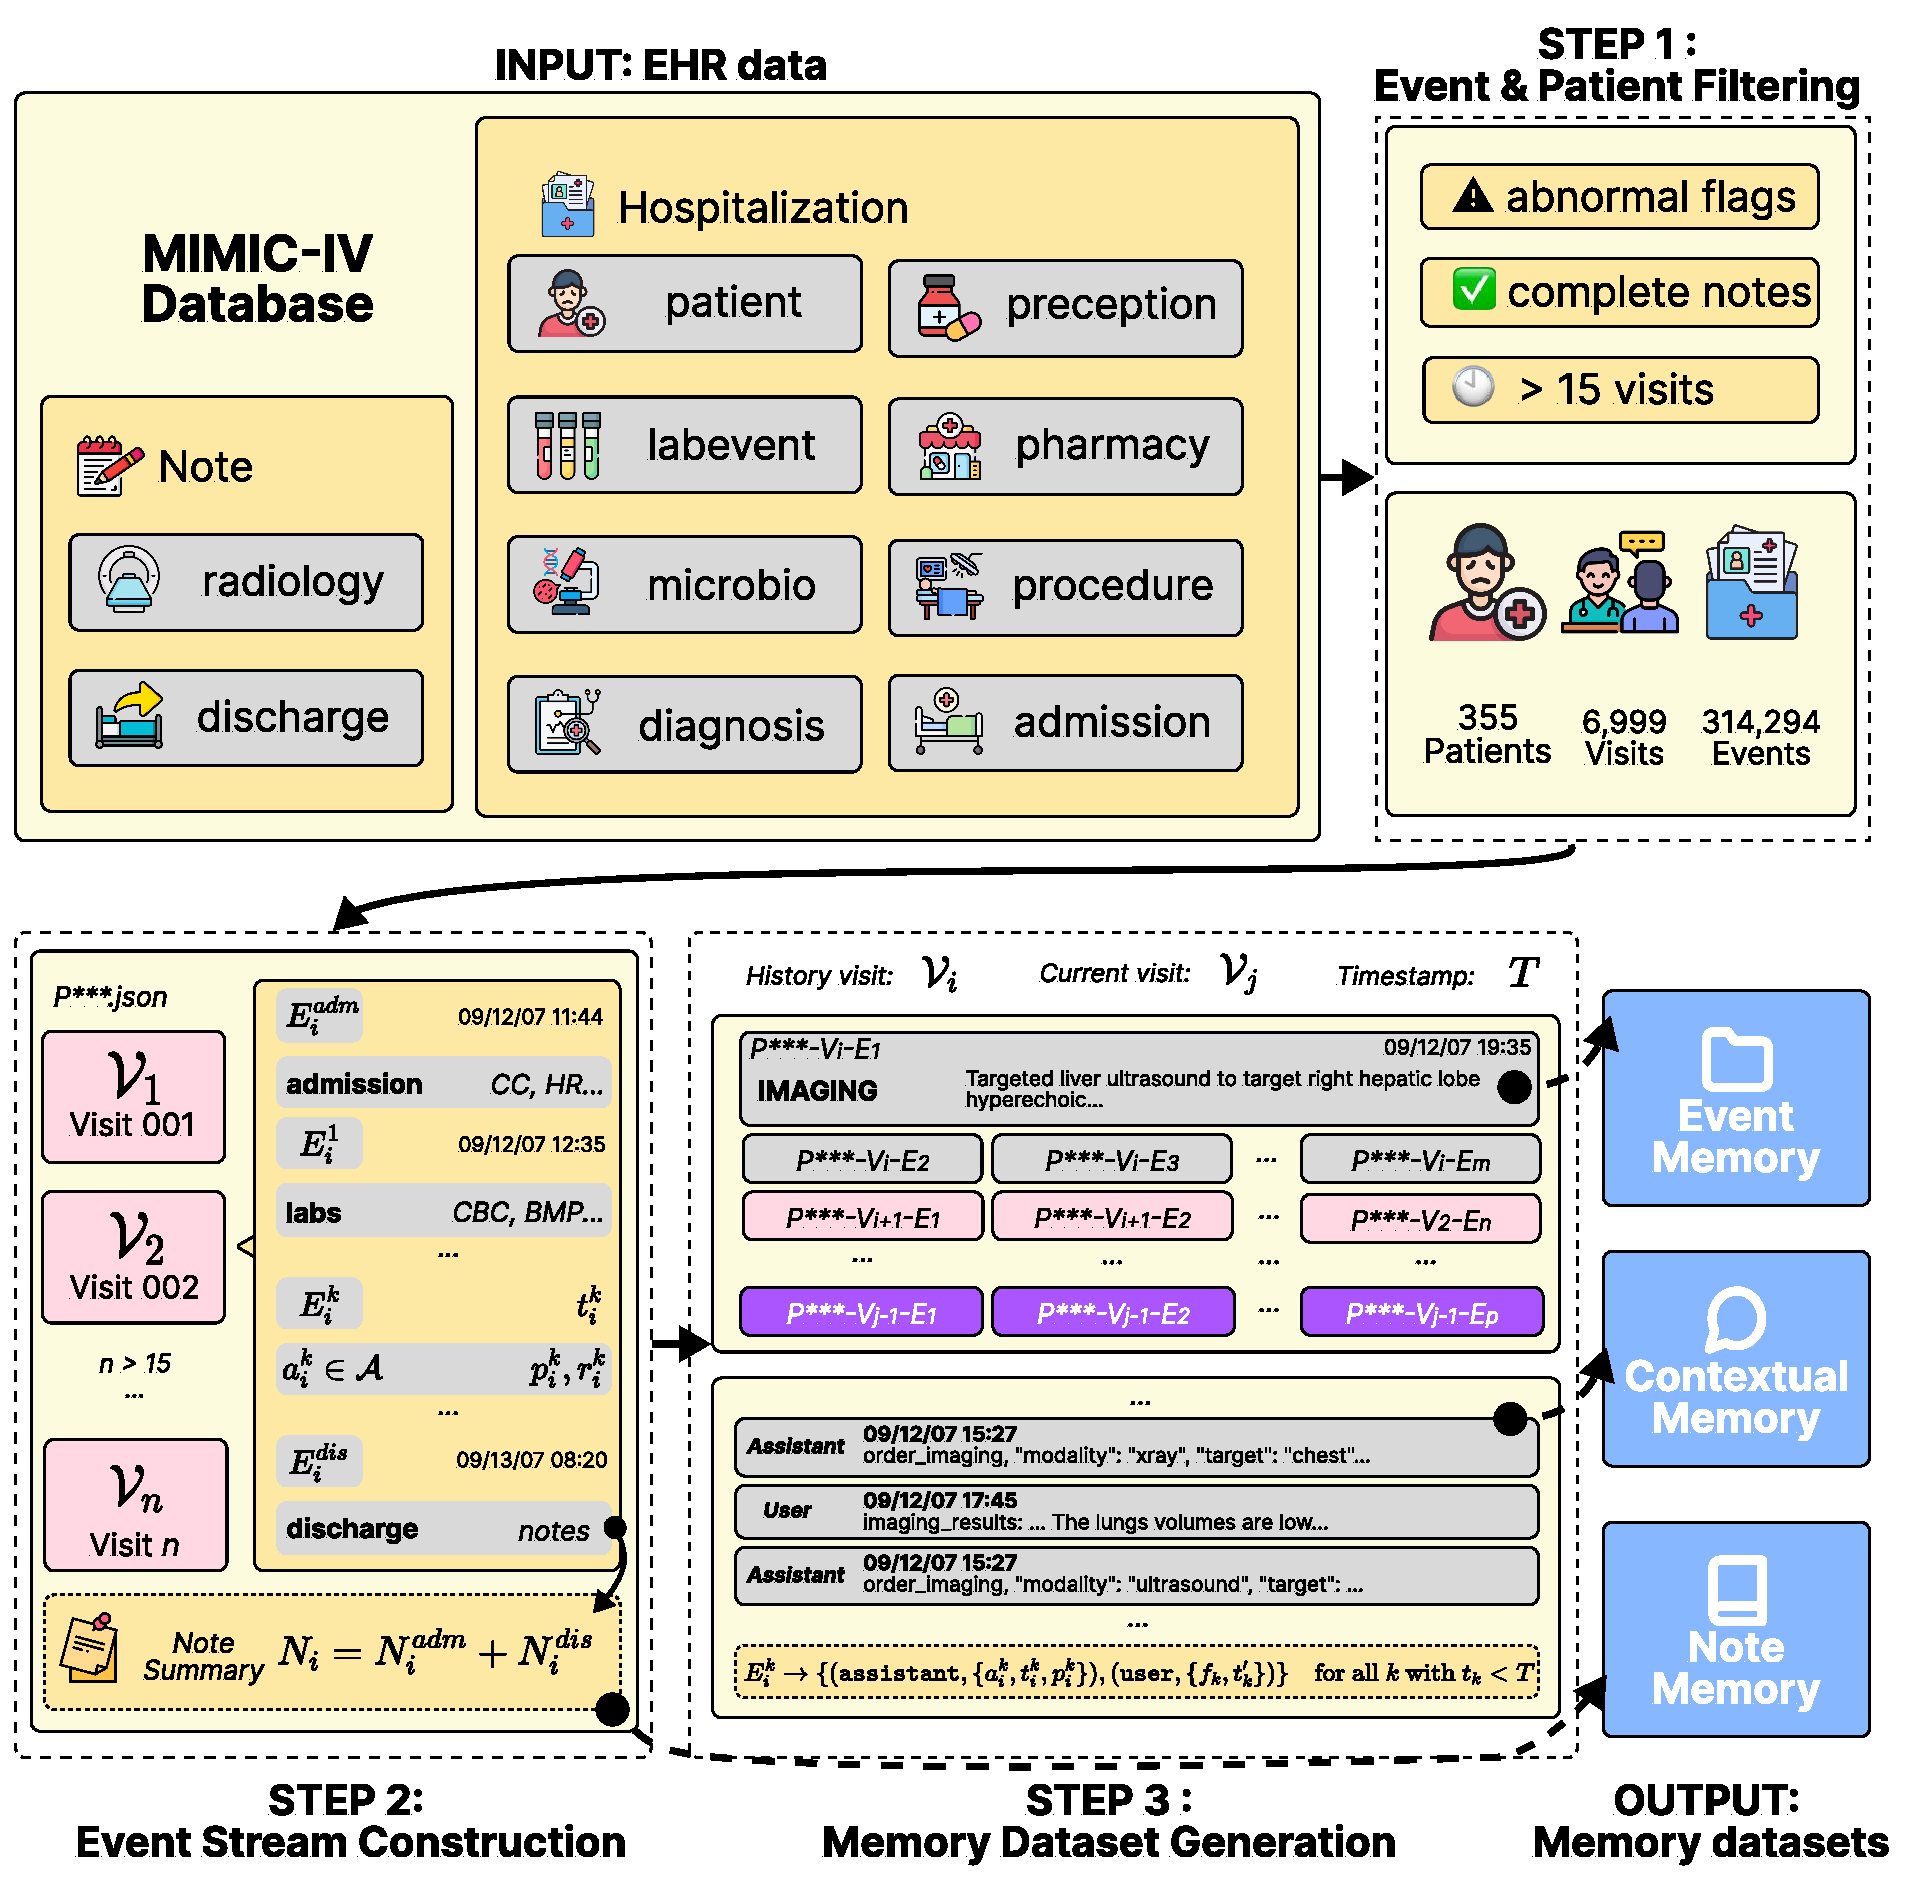
\includegraphics[width=\textwidth]{images/dataset_pipeline.pdf}
    \caption{Overview of the EHR data processing pipeline.}
    \label{fig:pipeline}
\end{figure}

LongMedBench is constructed from MIMIC-IV v3.1 \cite{PhysioNet-mimiciv-3.1}, a publicly available de-identified database containing comprehensive clinical data for over 100,000 patients at Beth Israel Deaconess Medical Center (2008--2022). To convert this database into an interactive agent-compatible environment, we design a three-stage pipeline (Figure~\ref{fig:pipeline}).


\subsection{Data Preprocessing \& Event Filtering}

\paragraph{Event-Level Filtering.} All structured clinical events are extracted from the \texttt{hosp} module, including laboratory measurements, microbiology cultures, medication prescriptions, pharmacy bills, diagnoses and procedures. Among these, we retain only laboratory results flagged as abnormal; normal lab values are excluded. Other events are retained in full. The rationale for this selective filtering strategy is discussed in Chapter~3.

From the \texttt{admissions} table, we decompose each hospitalization into two boundary events. The admission event captures the patient's demographics, chief complaint, and initial physical examination findings at intake. The discharge eventcaptures the discharge narrative and the final diagnoses recorded in \texttt{diagnoses\_icd}. 

\paragraph{Patient-Level Preprocessing.} We require each hospitalization to have a complete discharge summary from the \texttt{note} module whose timestamp aligns with the corresponding admission record in \texttt{hosp/admissions}; visits lacking a matched discharge note are excluded. From the remaining visits, we select patients with at least 15 recorded hospitalizations. The rationale for these filtering decisions is discussed in Chapter~3. 

\paragraph{Note Preprocessing.} Radiology reports are converted to structured imaging events via regular expression parsing: the modality \textit{(e.g., CT, X-ray, MRI)} and body region \textit{(e.g., chest, abdomen)} are extracted as the action type and parameter, respectively, while the full report text is retained as the observation result. Discharge notes $N_i$ are decomposed into admission information $N_i^{adm}$ and discharge information $N_i^{dis}$, then attached to the corresponding admission or discharge events. Both summaries are preserved in narrative format for use in Note Memory (Section~\ref{sec:notemem}) and ground-truth extraction. 

\paragraph{Resulting Cohort.} The filtered dataset comprises 355 patients with 6,999 inpatient visits. Mean visits per patient: 19.72 (median = 18.00, SD = 5.72). Mean medical events per visit: 44.91 (median = 25.00, SD = 70.32). The distribution of data is shown in Figure~\ref{fig:visit_distribution}. This dense multi-session structure challenges models on cross-visit memory retention and temporal reasoning.

\begin{figure}[ht]
    \centering
    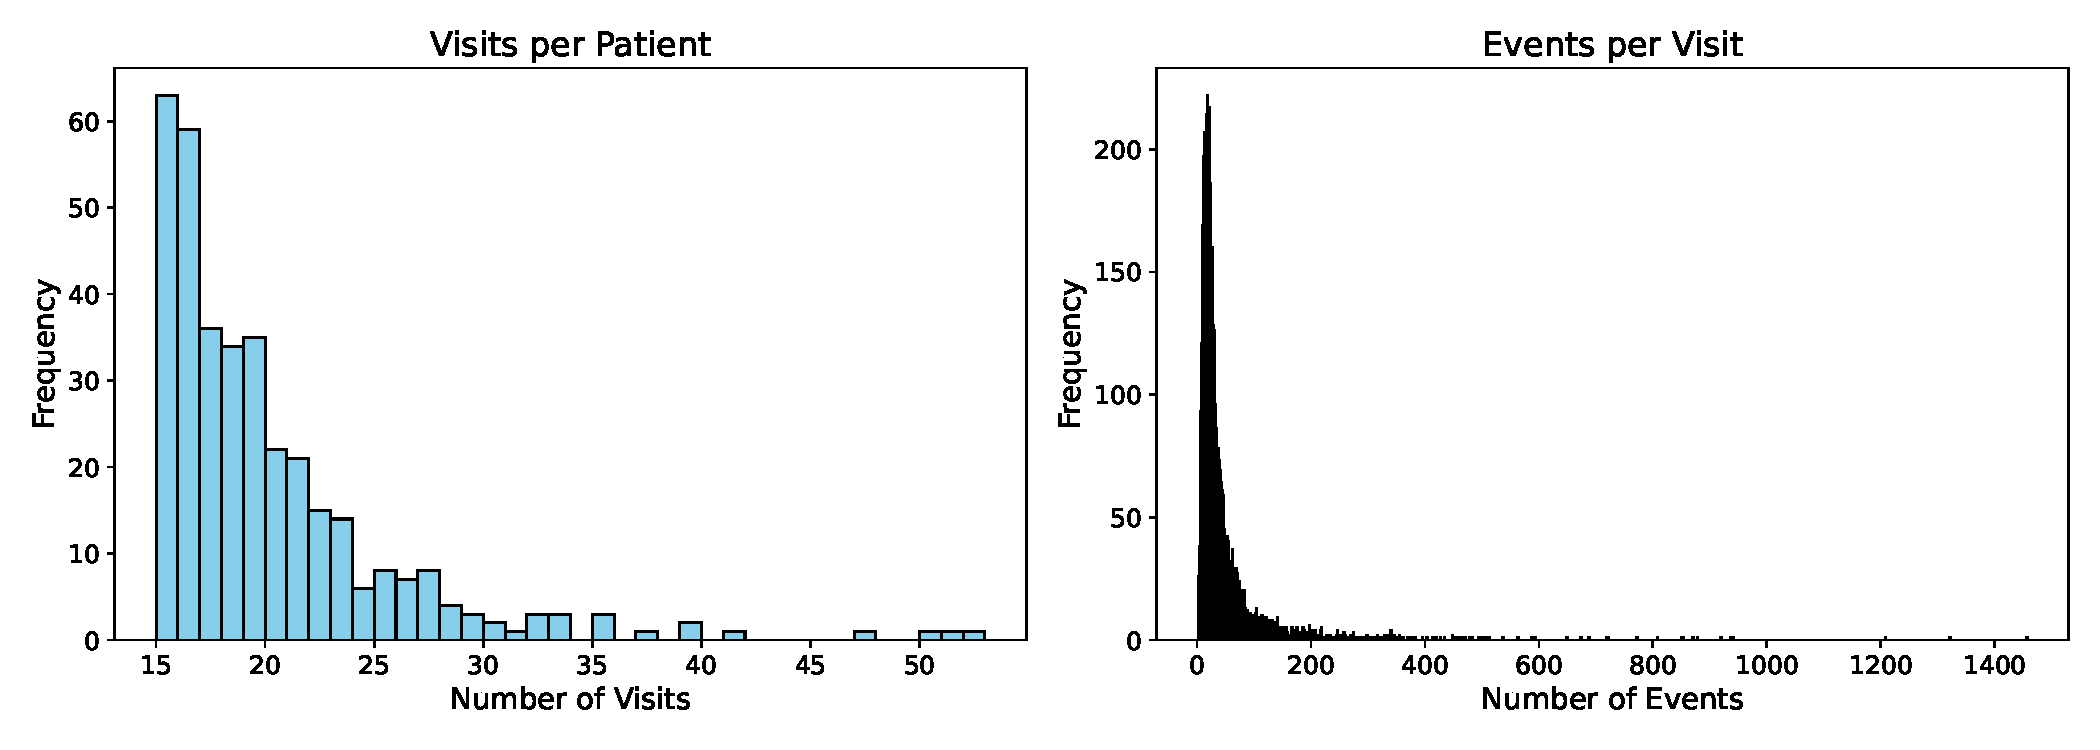
\includegraphics[width=\textwidth]{images/visit_distribution.pdf}
    \caption{Distribution of visits per patient in the filtered cohort.}
    \label{fig:visit_distribution}
\end{figure}

\subsection{Event Stream Construction}

We transform filtered records into a unified, time-ordered event stream for each patient. A medical event is any discrete clinical occurrence extracted from the structured hospitalization data. Formally, the $k_\text{th}$ event in $\mathcal{V}_i$ is $E^k_i := \{a^k_i, t^k_i, p^k_i, o^k_i\}$, where $a^k_i$ is the action type from the clinical action space $\mathcal{A}$, \textit{including imaging, lab tests, medication, etc.}, $t^k_i$ is the timestamp, $p^k_i$ is the action parameter \textit{(e.g., CT, X-ray, etc. for imaging)}, and $o^k_i$ is the observation result \textit{(e.g., a radiology report)}.

We define a visit as the period spanning from an admission event $E^{adm}_i$ to the corresponding discharge event $E^{dis}_i$. All other structured events occurring between these two timestamps are collected and ordered chronologically. Formally, each visit $\mathcal{V}_i$ can be represented as $\mathcal{V}_i = \{E^{adm}_i, E^1_i, E^2_i, \dots, E^m_i, E^{dis}_i\}$. The complete patient stream can therefore be denoted as $\mathcal{S_P} = \{\mathcal{V}_1, \mathcal{V}_2, \dots, \mathcal{V}_n\}$, where $n$ is the total number of visits.

\section{Three-Tier Memory Architecture}
\label{sec:memory}

To provide the agents with controlled provision of historical information, we define a three-tier memory architecture that systematically varies the granularity of historical information. Given the earliest historical visit $\mathcal{V}_i$, the current visit $\mathcal{V}_j$, and the current timestamp $T$, the agent's memory access is strictly bounded to prevent event leakage.

\subsection{Note Memory}
\label{sec:notemem}

$\mathcal{M}^{(i,j)}_N := \{N_i, N_{i+1}, \dots, N_{j-1}\}$, which contains continuous visit-level discharge summaries from $\mathcal{V}_i$ to $\mathcal{V}_{j-1}$. Note Memory is compact and preserves clinical narrative structure, emphasizing the global trajectory, but discards fine-grained temporal and event-level details.

\subsection{Event Memory}
\label{sec:eventmem}

$\mathcal{M}^{(i,j)}_E := \bigcup_{k=i}^{j-1} \mathcal{V}_k$, which contains all clinical events from $\mathcal{V}_i$ to $\mathcal{V}_{j-1}$. Events are flattened into a single chronological sequence, discarding visit-level boundaries and forming a unified trajectory. Event Memory is information-complete, and its volume creates a natural stress test for both long-context capabilities and retrieval strategies.

\subsection{Context Memory}
\label{sec:contextmem}

$\mathcal{M}_C^{(j,T)} := \{(r_0, m_0), (r_1, m_1), \dots, (r_P, m_P)\}$, where $r_k$ and $m_k$ denote the dialog role (\texttt{assistant} or \texttt{user}) and message content, respectively. Rewritten by LLM, any event $E_j^k$ in $\mathcal{V}_j$ with timestamp $t_j^k < T$ is transformed into a conversation trajectory between the agent and the clinical environment, simulating the agent's instant interaction state up to the decision point. 

Context Memory represents the baseline information always available to the agent. Historical memory ($\mathcal{M}^{(i,j)}_N$ or $\mathcal{M}^{(i,j)}_E$) is the experimental variable, enabling isolation of the marginal contribution of history beyond the immediate clinical context.

\section{Long-Horizon Decision-Making Task}
\label{sec:task}

\subsection{Task Formulation}

For a sampled ground-truth event $E_i^{GT}$ in the current visit $\mathcal{V}_i$ with timestamp $t_i^{GT}$, the working context is defined as $S=\mathcal{M}_C^{(i,t_i^{GT})}$, containing all interaction history available before the target event. The long-horizon memory is denoted as $M=\mathcal{M}^{(1,n)}_E$ or $M=\mathcal{M}^{(1,n)}_N$, depending on whether Event Memory or Note Memory is injected. At inference time, the agent receives $S$, an instructional prompt, $M$, and a multiple-choice query $Q$, then outputs an answer $\hat{y}$. The three subtasks are defined as follows:
\begin{itemize}
    \item   \textbf{Next Action Prediction} asks the agent to predict the future event action type $a_i^{GT}$ from the clinical action space $\mathcal{A}$.
    \item   \textbf{Argument Prediction} asks the agent to predict the target event argument $p_i^{GT}$, such as which laboratory panels or imaging modality are most appropriate.
    \item   \textbf{Discharge Decision} asks whether the patient should be discharged within $6$ hours, yielding a binary Yes/No decision.
\end{itemize}

\begin{figure}
    \centering
    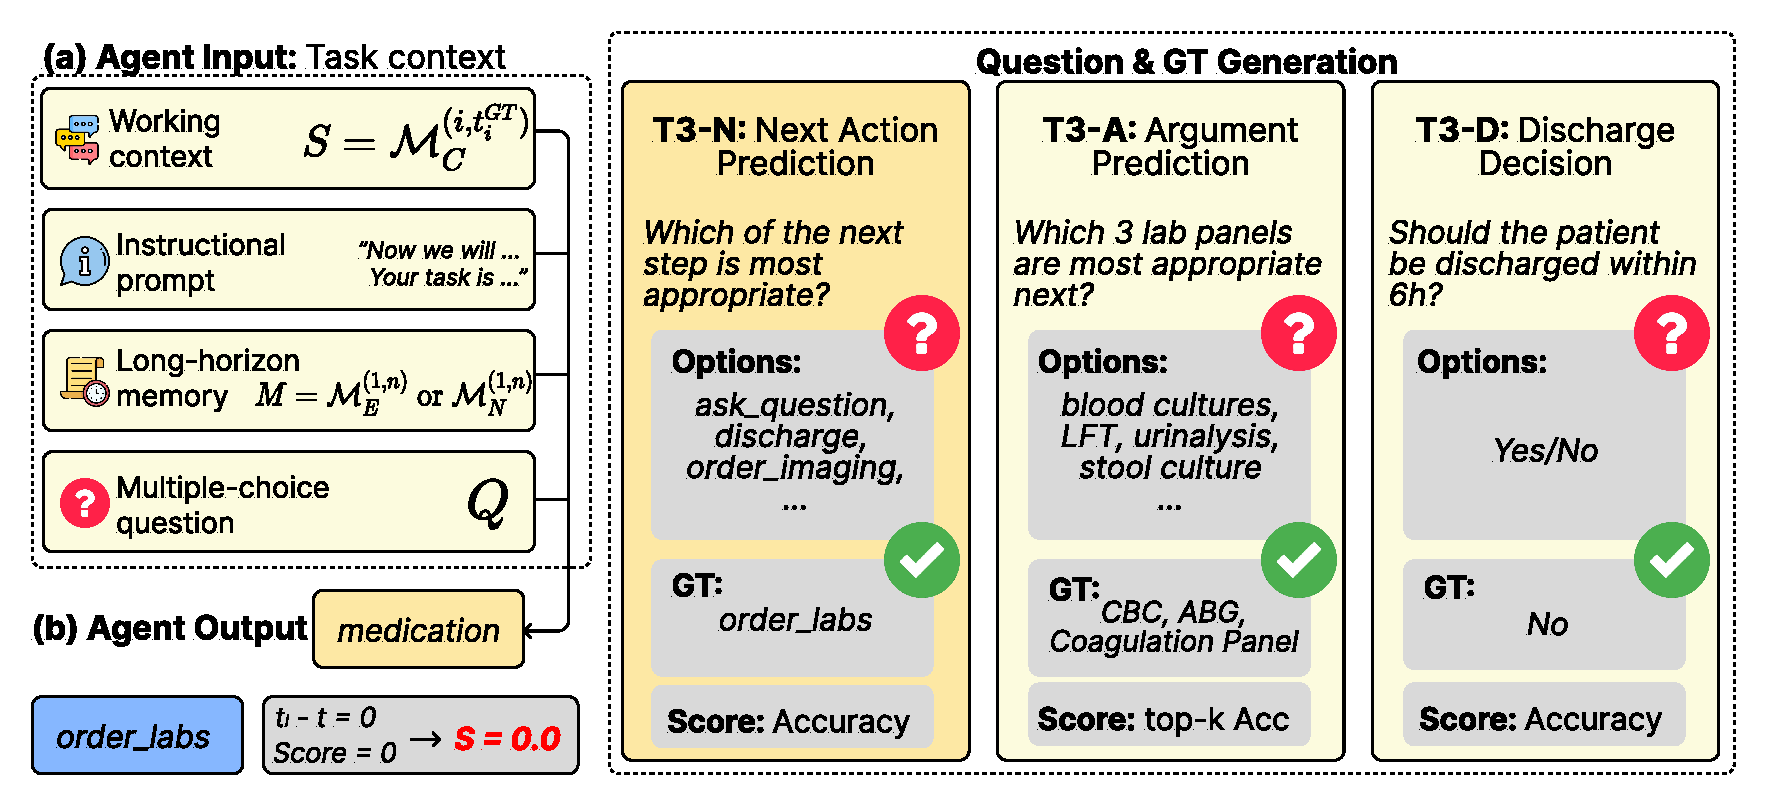
\includegraphics[width=\textwidth]{images/decision_making.pdf}
    \caption{Illustration of the long-horizon decision-making task.}
    \label{fig:decision_task}
\end{figure}

\subsection{Evaluation Metrics}

Next Action Prediction and Discharge Decision are evaluated by classification accuracy, while Argument Prediction is evaluated by top-$k$ accuracy because multiple arguments may be clinically appropriate. For Next Action Prediction and Argument Prediction, LongMedBench additionally applies a time-decay scoring mechanism to avoid over-penalizing decisions whose equivalent ground-truth action occurs shortly after the sampled timestamp. Let
\[
\mathcal{E}_{24h}=\{E_i^k \mid t_i^k\in[t_i^{GT},t_i^{GT}+24\mathrm{h}]\}.
\]
The score is
\[
S=\max_{E_i^k\in\mathcal{E}_{24h}}
\exp\{-\lambda(t_i^k-t_i^{GT})\}\cdot\operatorname{Score}(y_i^k,\hat{y}),
\quad
\lambda=\frac{\ln(100)}{24},
\]
where the decay factor decreases from $1.0$ at the target timestamp to $0.01$ after $24$ hours, $\operatorname{Score}(\cdot)$ is classification accuracy for Next Action Prediction and top-$k$ accuracy for Argument Prediction. Discharge Decision is evaluated directly as binary classification accuracy.

\section{Experimental Setup}
\label{sec:expsetup}

\subsection{Models}

We evaluate three state-of-the-art LLMs: GPT-5-mini, DeepSeek-v3.2 (with and without reasoning mode), and Qwen-Turbo. All are evaluated through their respective APIs with standardized prompts and default model configurations.

\subsection{Agent Architectures}

Given the fixed memory modules $\{\mathcal{M}^{(i,j)}_N, \mathcal{M}^{(i,j)}_E, \mathcal{M}_C^{(j,T)}\}$, three strategies control how historical memory is provided to the agent: \textbf{ (1) Naive Long-Context (Baseline).} $\mathcal{M}^{(i,j)}_N$ or $\mathcal{M}^{(i,j)}_E$ is provided in full within the model's context window alongside $\mathcal{M}_C^{(j,T)}$, testing native long-context attention without external retrieval assistance. \textbf{ (2) RAG.} $\mathcal{M}^{(i,j)}_N$ or $\mathcal{M}^{(i,j)}_E$ is externally indexed. At decision time, $\mathcal{M}_C^{(j,T)}$ serves as the retrieval query; top-$k$ relevant chunks are retrieved and concatenated with the context. This tests whether selective retrieval overcomes lost-in-the-middle effects. \textbf{(3) Agent Memory System.} We integrate the Mem0 framework \cite{mem0_reference}, providing a persistent, evolvable memory store to the agent. The agent can add, search, and update memory across a patient's trajectory, actively managing what is stored and retrieved. This tests whether agentic memory management outperforms passive retrieval.

\subsection{Experimental Conditions}

We design a factorial ablation varying four factors:

\begin{enumerate}
    \item \textbf{Memory Granularity:} Note Memory vs.\ Event Memory.
    \item \textbf{Provision Strategy:} Naive Long-Context vs.\ RAG vs.\ Mem0.
    \item \textbf{Historical Depth ($n$):} Number of injected historical visits: $n \in \{0, 1, 2, 3, \infty\}$. $n=0$ provides Context Memory $\mathcal{M}_C^{(j,T)}$ only (no history) as baseline.
    \item \textbf{Reasoning Mode:} Standard vs.\ chain-of-thought (DeepSeek-v3.2 only).
\end{enumerate}

Qwen-Turbo serves as the primary ablation vehicle; key conditions are replicated on GPT-5-mini and DeepSeek-v3.2 for cross-model validation.

\section{Results and Analysis}
\label{sec:results}

\subsection{Overall Decision-Making Performance Across Subtasks}

Table~\ref{tab:decision_overall} summarizes long-horizon decision-making performance under the naive long-context setting. We report all three decision-making subtasks rather than treating Discharge Decision as the entire benchmark. Across models, Discharge Decision is consistently easier than Next Action Prediction, while Argument Prediction falls between them. This separation is important: high discharge-decision accuracy does not imply strong action planning or argument selection.

\begin{table}[!h]
    \centering
    \caption{Long-context LLM performance on long-horizon decision-making. Argument evaluates event argument prediction, Discharge evaluates six-hour discharge decision, and Action evaluates next action-type prediction.}
    \label{tab:decision_overall}
    {\fontsize{8}{9.2}\selectfont
    \setlength{\tabcolsep}{2pt}
    \renewcommand{\arraystretch}{1.05}
    \begin{tabular*}{\textwidth}{l@{\extracolsep{\fill}}cccccccc}
        \toprule
        & \multicolumn{4}{c}{\textbf{Note Memory}} & \multicolumn{4}{c}{\textbf{Event Memory}} \\
        \cmidrule(lr){2-5}\cmidrule(lr){6-9}
        \textbf{Model} & \textbf{Argument} & \textbf{Discharge} & \textbf{Action} & \textbf{Avg} & \textbf{Argument} & \textbf{Discharge} & \textbf{Action} & \textbf{Avg} \\
        \midrule
        Qwen-Turbo & 0.475 & 0.604 & 0.309 & 0.434 & 0.494 & 0.604 & 0.309 & 0.420 \\
        DeepSeek-v3.2 & 0.478 & 0.607 & 0.278 & 0.422 & 0.493 & 0.607 & 0.304 & 0.439 \\
        GPT-5-mini & 0.478 & 0.625 & 0.324 & 0.445 & 0.494 & 0.607 & 0.335 & 0.452 \\
        DeepSeek-v3.2-thinking & 0.471 & 0.578 & 0.294 & 0.420 & 0.466 & 0.593 & 0.290 & 0.419 \\
        \bottomrule
    \end{tabular*}}
\end{table}

\subsection{Subtask-Level Patterns}

The most visible pattern is that Discharge Decision should not be interpreted as the whole decision-making task. It reaches approximately 0.58--0.63 because it is a binary discharge decision, whereas Next Action Prediction remains around 0.28--0.34 because selecting the next action type requires finer-grained clinical planning. Argument Prediction lies in the middle, reflecting the difficulty of selecting appropriate event arguments such as laboratory panels or imaging targets. Event Memory slightly improves Argument Prediction in most models, suggesting that fine-grained historical events help parameter selection, but the gains do not consistently translate into higher average decision-making performance.

\subsection{Memory Ablations: Visit Injection and Retrieval Architectures}

Table~\ref{tab:decision_ablation} reports the Qwen-Turbo ablation used to test historical depth and memory-augmentation strategies. The $n=0$ setting provides only Context Memory $\mathcal{M}_C^{(j,T)}$ and no injected historical memory. Increasing the number of injected visits does not produce monotonic gains, and retrieval-based architectures remain close to or below the naive baseline.

\begin{table}[!h]
    \centering
    \caption{Ablation study on long-horizon decision-making using Qwen-Turbo. The left block varies injected visit history; the right block compares retrieval/memory architectures.}
    \label{tab:decision_ablation}
    {\fontsize{8}{9.2}\selectfont
    \setlength{\tabcolsep}{4pt}
    \renewcommand{\arraystretch}{1.05}
    \begin{tabular*}{\textwidth}{ll@{\extracolsep{\fill}}cccc}
        \toprule
        \textbf{Setting} & \textbf{Memory/Arch} & \textbf{Argument} & \textbf{Discharge} & \textbf{Action} & \textbf{Avg} \\
        \midrule
        \multicolumn{6}{l}{\textbf{Visit Injection}} \\
        $n=0$ & -- & 0.49 & 0.61 & 0.32 & 0.45 \\
        $n=2$ & Event & 0.49 & 0.60 & 0.32 & 0.44 \\
        $n=5$ & Event & 0.48 & 0.60 & 0.31 & 0.43 \\
        $n=2$ & Note & 0.48 & 0.60 & 0.32 & 0.44 \\
        $n=5$ & Note & 0.48 & 0.60 & 0.32 & 0.44 \\
        \midrule
        \multicolumn{6}{l}{\textbf{Memory Architecture}} \\
        RAG & Event & 0.45 & 0.51 & 0.29 & 0.40 \\
        Mem0 & Event & 0.47 & 0.62 & 0.31 & 0.44 \\
        RAG & Note & 0.48 & 0.60 & 0.31 & 0.44 \\
        Mem0 & Note & 0.46 & 0.56 & 0.29 & 0.41 \\
        \bottomrule
    \end{tabular*}}
\end{table}

\textbf{Finding.} The ablation results revise the earlier interpretation: the negative result is not specific to Discharge Decision, but spans the broader decision-making suite. Even when historical information is made available through longer visit injection, RAG, or Mem0, models do not systematically improve on Argument Prediction, Discharge Decision, or Next Action Prediction. The $n=0$ baseline remains competitive, indicating that agents rely heavily on immediate context and struggle to convert retrieved history into better decisions.

\subsection{Chain-of-Thought Reasoning}

Explicit chain-of-thought reasoning does not improve decision-making performance for DeepSeek-v3.2. Under Event Memory, the average score drops from 0.439 to 0.419, and Discharge Decision decreases from 0.607 to 0.593. This suggests that reasoning mode may make the model more conservative or distract it from committing to the multiple-choice decision, especially when the task requires selecting an actionable next step rather than explaining uncertainty.

\subsection{Summary of Findings}

The experimental results converge on a refined narrative: (1) decision-making remains challenging, especially for Next Action Prediction; (2) Discharge Decision is easier and should not be used as a proxy for the entire decision-making benchmark; (3) Event Memory can modestly improve Argument Prediction but does not reliably improve average decision-making performance; (4) historical visit injection, RAG, and Mem0 do not provide systematic gains over the immediate-context baseline; and (5) chain-of-thought reasoning can degrade performance through increased conservatism. These findings collectively reveal a retrieval-reasoning gap whose implications we explore in Chapter~3.

\subsection{Qualitative Case Studies}

To ground the quantitative results in concrete agent behaviors, we inspect representative decision instances from the evaluation set. The following cases illustrate how memory architecture and memory type shape agent decisions at the level of individual queries.

\paragraph{Historical memory can change answers---sometimes for the worse.}
In a Next Action Prediction instance for a chemotherapy patient (Patient~3, Visit~16), the ground-truth next action is \texttt{medication}. With no injected history ($n=0$), the agent correctly selects \texttt{medication}, reasoning that furosemide is needed to manage fluid overload during chemotherapy. At $n=2$, the same correct answer is produced. However, at $n=5$, the agent switches to \texttt{order\_labs}, now reasoning that ``the patient is undergoing R-ICE chemotherapy and has abnormal lab results, indicating the need for further laboratory testing.'' Five historical visits introduce enough distracting context to overrule the initially correct decision. This non-monotonic pattern---correct at moderate history, wrong at longer history---mirrors the aggregate ablation results and suggests that longer context can dilute rather than strengthen clinical judgment.

\paragraph{Retrieved history can mislead when it mimics the current presentation.}
In an Argument Prediction instance (Patient~1, Visit~20), the agent must select the most appropriate next imaging study for a patient with bilateral lower-extremity edema. The long-context baseline correctly selects \texttt{XRAY abdomen}, reasoning that systemic conditions such as liver disease or heart failure warrant abdominal evaluation. The RAG-augmented agent selects \texttt{CT chest}, distracted by retrieved note text mentioning chest pain and a non-diagnostic chest X-ray. The Mem0-augmented agent selects \texttt{CT head}, focusing on a retrieved headache complaint from an earlier visit. Both retrieval-based agents are led astray by historical snippets that superficially match but are clinically irrelevant to the current presentation. This illustrates a concrete failure mode: when retrieval returns temporally nearby but causally unrelated events, the agent conflates them with the immediate clinical context.

\paragraph{Note Memory can misattribute retrieved content to the current visit.}
In another Next Action Prediction instance (Patient~1, Visit~20), the ground-truth action is \texttt{order\_labs}. The Mem0 agent correctly selects \texttt{order\_labs} under Event Memory, citing persistent electrolyte abnormalities and rising creatinine. Under Note Memory, however, the same agent switches to \texttt{medication}, justifying the choice with a positive stool culture for \textit{Salmonella} found in a retrieved discharge summary from a prior admission. The agent fails to distinguish a retrospective finding from a current clinical need, treating historical note content as actionable evidence for the present visit. This confusion is less likely under Event Memory, where explicit timestamps and structured fields make temporal provenance clearer.

\subsection{Discussion of Negative Results}

The finding that memory augmentation does not improve decision-making may appear discouraging, but it carries productive implications. First, it identifies a genuine capability gap that current architectures cannot bridge through scale or retrieval quality alone---the gap is architectural, not parametric. Second, it provides a clear target for future work: architectures that explicitly model the relationship between retrieved history and current decisions, rather than treating retrieval as an independent preprocessing step. Third, the qualitative cases reveal specific failure modes---context dilution at longer histories, distraction by superficially similar retrieved snippets, and temporal misattribution of note content---that are diagnosable and potentially addressable through memory designs that preserve temporal provenance and causal relevance.

The contrast with EHR-Bench \cite{2025_ehr_r1} is instructive. EHR-Bench demonstrated that LLMs can predict next clinical events from complete histories with non-trivial accuracy, but our agent-based setting reveals that this does not translate to interactive decision-making where history must be selectively retrieved and integrated. The two paradigms evaluate complementary but distinct capabilities---static prediction vs.\ interactive planning---and the gap between them highlights the importance of evaluation methodology in assessing clinical AI readiness.
